%
% $RCSfile: model_metamorphosis.tex,v $
%
% Copyright (C) 2002-2008. Christian Heller.
%
% Permission is granted to copy, distribute and/or modify this document
% under the terms of the GNU Free Documentation License, Version 1.1 or
% any later version published by the Free Software Foundation; with no
% Invariant Sections, with no Front-Cover Texts and with no Back-Cover
% Texts. A copy of the license is included in the section entitled
% "GNU Free Documentation License".
%
% http://www.cybop.net
% - Cybernetics Oriented Programming -
%
% http://www.resmedicinae.org
% - Information in Medicine -
%
% Version: $Revision: 1.1 $ $Date: 2008-08-19 20:41:07 $ $Author: christian $
% Authors: Christian Heller <christian.heller@tuxtax.de>
%

\subsection{Model Metamorphosis}
\label{model_metamorphosis_heading}
\index{Model Metamorphosis}
\index{Metamorphosis of Models}

One way to recognise the importance of \emph{Composition}, that is of models
with hierarchical character, is to compare several traditional modelling
approaches, as first suggested by Thomas Beale in \cite[p. 11-18]{archetypes}.
This \emph{Metamorphosis of Models} is empathised in the following paragraphs.

%
% $RCSfile: single_model.tex,v $
%
% Copyright (C) 2002-2008. Christian Heller.
%
% Permission is granted to copy, distribute and/or modify this document
% under the terms of the GNU Free Documentation License, Version 1.1 or
% any later version published by the Free Software Foundation; with no
% Invariant Sections, with no Front-Cover Texts and with no Back-Cover
% Texts. A copy of the license is included in the section entitled
% "GNU Free Documentation License".
%
% http://www.cybop.net
% - Cybernetics Oriented Programming -
%
% http://www.resmedicinae.org
% - Information in Medicine -
%
% Version: $Revision: 1.1 $ $Date: 2008-08-19 20:41:08 $ $Author: christian $
% Authors: Christian Heller <christian.heller@tuxtax.de>
%

\subsubsection{Single Model}
\label{single_model_heading}
\index{Single Model Approach}
\index{Entity Relationship Model}
\index{ERM}
\index{Object Oriented Model}
\index{OOM}
\index{Unified Modelling Language}
\index{UML}

Today, the most common design approach for standard application software is to
create a \emph{Single Model} of types whose semantics is often described in
form of an \emph{Entity Relationship-} (ER) or \emph{Object Oriented} (OO)
model,
%(section \ref{data_model_heading}),
the latter sometimes illustrated
using diagrams of the \emph{Unified Modeling Language} (UML).

\begin{figure}[ht]
    \begin{center}
        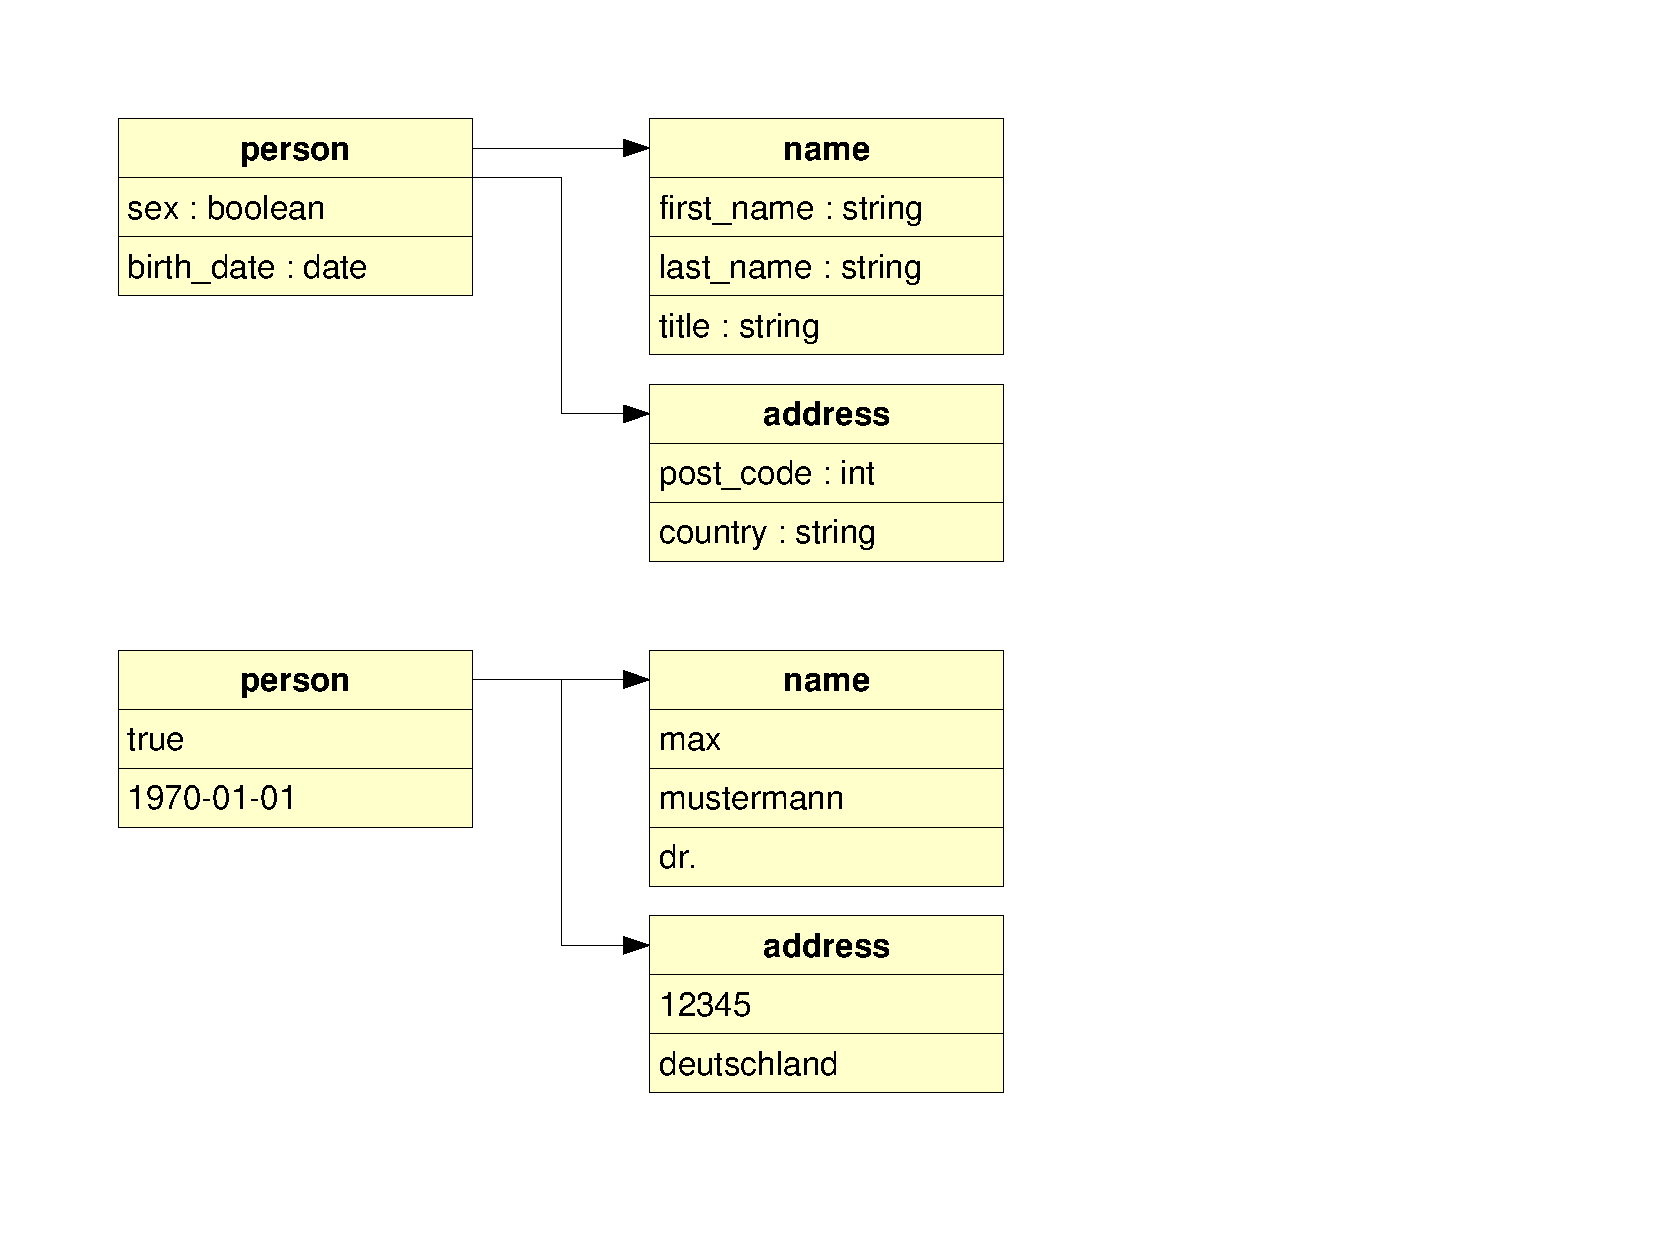
\includegraphics[scale=0.3,angle=-90]{graphic/single.pdf}
        \caption{Single Model Approach (adapted from \cite{archetypes})}
        \label{single_figure}
    \end{center}
\end{figure}

As example, figure \ref{single_figure} shows a UML \emph{Class Diagram} (CsD).
In its upper half, one can see a class \emph{Person} associated with the
classes \emph{Name} and \emph{Address}, as modelled at design time. They may be
part of a much larger model. The lower half of the figure shows the objects
(instances) at runtime, filled with concrete values. There are a number of
problems with this approach:

%
% $RCSfile: inflexible_architecture.tex,v $
%
% Copyright (C) 2002-2008. Christian Heller.
%
% Permission is granted to copy, distribute and/or modify this document
% under the terms of the GNU Free Documentation License, Version 1.1 or
% any later version published by the Free Software Foundation; with no
% Invariant Sections, with no Front-Cover Texts and with no Back-Cover
% Texts. A copy of the license is included in the section entitled
% "GNU Free Documentation License".
%
% http://www.cybop.net
% - Cybernetics Oriented Programming -
%
% http://www.resmedicinae.org
% - Information in Medicine -
%
% Version: $Revision: 1.1 $ $Date: 2008-08-19 20:41:07 $ $Author: christian $
% Authors: Christian Heller <christian.heller@tuxtax.de>
%

\paragraph{Inflexible Architecture}
\label{inflexible_architecture_heading}
\index{Inflexible Architecture}

First and foremost, the static coupling of classes leads to an inflexible
design. The names and number of attributes and methods as integral part of a
class cannot be changed dynamically later-on; only their values can. The class
structure represents a solution to a current problem. If it is static, then
future requirements cannot be considered. Adaptation issues and workarounds,
affecting stability and security, are thus to be expected.

%
% $RCSfile: concept_mix.tex,v $
%
% Copyright (C) 2002-2008. Christian Heller.
%
% Permission is granted to copy, distribute and/or modify this document
% under the terms of the GNU Free Documentation License, Version 1.1 or
% any later version published by the Free Software Foundation; with no
% Invariant Sections, with no Front-Cover Texts and with no Back-Cover
% Texts. A copy of the license is included in the section entitled
% "GNU Free Documentation License".
%
% http://www.cybop.net
% - Cybernetics Oriented Programming -
%
% http://www.resmedicinae.org
% - Information in Medicine -
%
% Version: $Revision: 1.1 $ $Date: 2008-08-19 20:41:06 $ $Author: christian $
% Authors: Christian Heller <christian.heller@tuxtax.de>
%

\paragraph{Concept Mix}
\label{concept_mix_heading}
\index{Concept Mix}

Further, specialised domain concepts identified during requirements analysis
(such as a \emph{Patient} being a kind of \emph{Person}) are often mixed up
with more general concepts as found during design (for example the application
of a proper \emph{Role} architecture instead of simple inheritance for the
person-patient relation). The lack of a proper separation between pure domain
knowledge (like a patient receiving a medication) and system control software
(like logging facilities or persistence mechanisms) was already explained in
detail in the previous chapter \ref{statics_and_dynamics_heading}. It frequently
leads to strong coupling between system layers and complicates software design.

%
% $RCSfile: synchronisation_problems.tex,v $
%
% Copyright (C) 2002-2008. Christian Heller.
%
% Permission is granted to copy, distribute and/or modify this document
% under the terms of the GNU Free Documentation License, Version 1.1 or
% any later version published by the Free Software Foundation; with no
% Invariant Sections, with no Front-Cover Texts and with no Back-Cover
% Texts. A copy of the license is included in the section entitled
% "GNU Free Documentation License".
%
% http://www.cybop.net
% - Cybernetics Oriented Programming -
%
% http://www.resmedicinae.org
% - Information in Medicine -
%
% Version: $Revision: 1.1 $ $Date: 2008-08-19 20:41:09 $ $Author: christian $
% Authors: Christian Heller <christian.heller@tuxtax.de>
%

\paragraph{Synchronisation Problems}
\label{synchronisation_problems_heading}
\index{Synchronisation Problems}

The mix of application knowledge with system control software also causes
synchronisation (communication) problems within software development projects.
Domain experts and software developers depend on each other: Developers need to
first understand domain knowledge before being able to correctly implement it
into software. Experts bring their knowledge into a more software-friendly
form, during analysis.

%
% $RCSfile: complicated_processing.tex,v $
%
% Copyright (C) 2002-2008. Christian Heller.
%
% Permission is granted to copy, distribute and/or modify this document
% under the terms of the GNU Free Documentation License, Version 1.1 or
% any later version published by the Free Software Foundation; with no
% Invariant Sections, with no Front-Cover Texts and with no Back-Cover
% Texts. A copy of the license is included in the section entitled
% "GNU Free Documentation License".
%
% http://www.cybop.net
% - Cybernetics Oriented Programming -
%
% http://www.resmedicinae.org
% - Information in Medicine -
%
% Version: $Revision: 1.1 $ $Date: 2008-08-19 20:41:06 $ $Author: christian $
% Authors: Christian Heller <christian.heller@tuxtax.de>
%

\paragraph{Complicated Processing}
\label{complicated_processing_heading}
\index{Complicated Processing}
\index{Data Mining}
\index{Decision Support}

Due to the great variety of software architectures, it is pretty hard to
capture and process data from different systems in a uniform way, for reasons
of \emph{Data Mining}, for example. Unpredictable architecture changes caused
by new domain requirements hamper the creation of reliable rules for
\emph{Decision Support}.

%
% $RCSfile: steady_upgrading.tex,v $
%
% Copyright (C) 2002-2008. Christian Heller.
%
% Permission is granted to copy, distribute and/or modify this document
% under the terms of the GNU Free Documentation License, Version 1.1 or
% any later version published by the Free Software Foundation; with no
% Invariant Sections, with no Front-Cover Texts and with no Back-Cover
% Texts. A copy of the license is included in the section entitled
% "GNU Free Documentation License".
%
% http://www.cybop.net
% - Cybernetics Oriented Programming -
%
% http://www.resmedicinae.org
% - Information in Medicine -
%
% Version: $Revision: 1.1 $ $Date: 2008-08-19 20:41:09 $ $Author: christian $
% Authors: Christian Heller <christian.heller@tuxtax.de>
%

\paragraph{Steady Upgrading}
\label{steady_upgrading_heading}
\index{Steady Upgrading}

Applications that were designed in a \emph{Single Model} manner require steady
upgrading. Whenever new domain knowledge gets worked into the system or
existing knowledge gets adapted to new requirements, the software design may
change -- even in important parts that would better remain stable. Accordingly,
systems of that kind cannot be labelled \emph{future-proof}.

%
% $RCSfile: no_standardisation.tex,v $
%
% Copyright (C) 2002-2008. Christian Heller.
%
% Permission is granted to copy, distribute and/or modify this document
% under the terms of the GNU Free Documentation License, Version 1.1 or
% any later version published by the Free Software Foundation; with no
% Invariant Sections, with no Front-Cover Texts and with no Back-Cover
% Texts. A copy of the license is included in the section entitled
% "GNU Free Documentation License".
%
% http://www.cybop.net
% - Cybernetics Oriented Programming -
%
% http://www.resmedicinae.org
% - Information in Medicine -
%
% Version: $Revision: 1.1 $ $Date: 2008-08-19 20:41:07 $ $Author: christian $
% Authors: Christian Heller <christian.heller@tuxtax.de>
%

\paragraph{No Standardisation}
\label{no_standardisation_heading}
\index{Difficult Standardisation of Software Models}

Finally, a true standardisation of single model systems is hardly reachable.
Requirements are just too different between the systems, and they change much
too often. A standard architecture of that kind won't remain stable for very
long.


%
% $RCSfile: semi_structured_model.tex,v $
%
% Copyright (C) 2002-2008. Christian Heller.
%
% Permission is granted to copy, distribute and/or modify this document
% under the terms of the GNU Free Documentation License, Version 1.1 or
% any later version published by the Free Software Foundation; with no
% Invariant Sections, with no Front-Cover Texts and with no Back-Cover
% Texts. A copy of the license is included in the section entitled
% "GNU Free Documentation License".
%
% http://www.cybop.net
% - Cybernetics Oriented Programming -
%
% http://www.resmedicinae.org
% - Information in Medicine -
%
% Version: $Revision: 1.1 $ $Date: 2008-08-19 20:41:08 $ $Author: christian $
% Authors: Christian Heller <christian.heller@tuxtax.de>
%

\subsubsection{Semi Structured Model}
\label{semi_structured_model_heading}
\index{Semi Structured Model Approach}
\index{Named Values}
\index{Tagged Values}

A slightly improved version is the \emph{Semi Structured Model}. It relies on
the usage of \emph{Named Values} (sometimes called \emph{Tagged Values}), which
are stored in a dynamically extensible structure such as a list. That way,
future attributes can be added smoothly, without having to change the overall
model.

\begin{figure}[ht]
    \begin{center}
        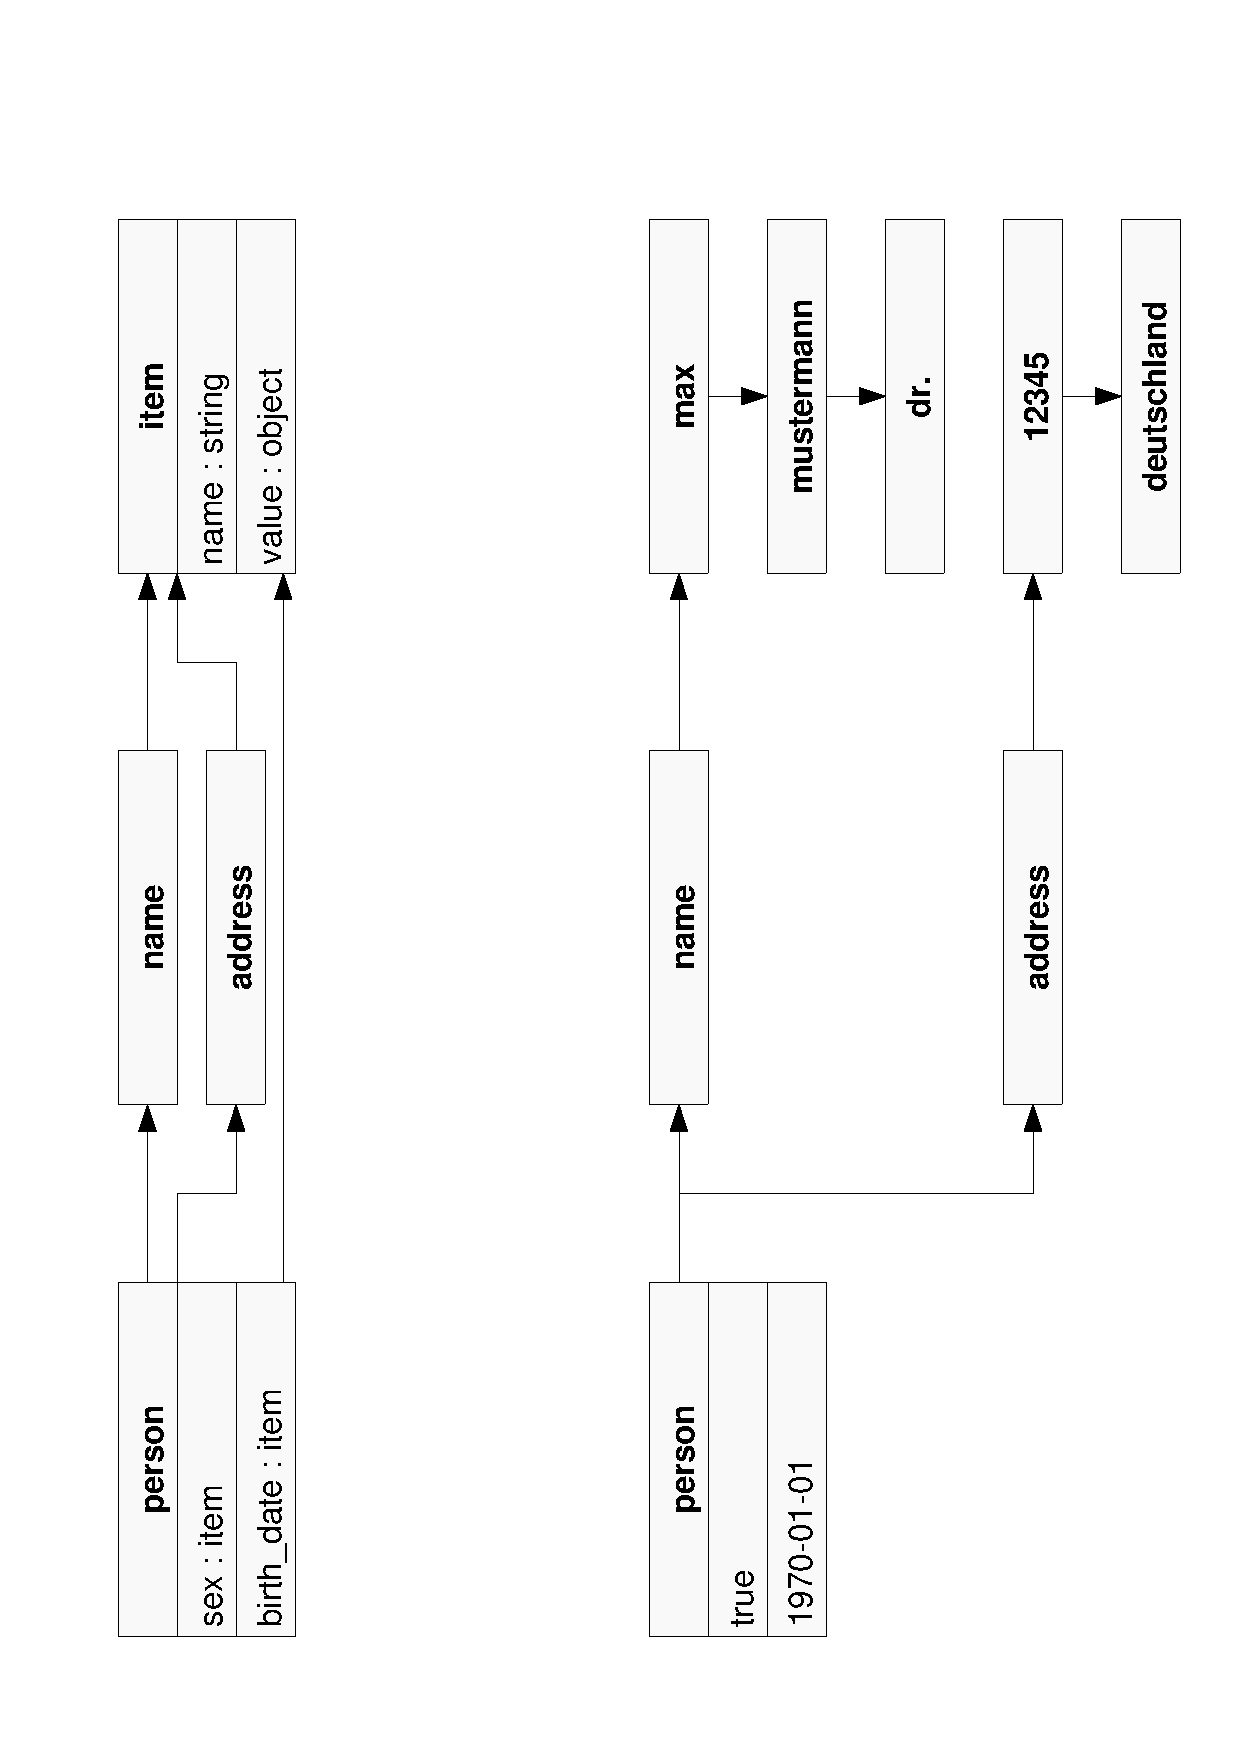
\includegraphics[scale=0.3,angle=-90]{graphic/semi.pdf}
        \caption{Semi Structured Model Approach (adapted from \cite{archetypes})}
        \label{semi_figure}
    \end{center}
\end{figure}

The example in figure \ref{semi_figure} shows a class \emph{Person} referencing
two linked lists, one called \emph{Name} and another called \emph{Address}. The
list elements are of type \emph{Item}. The dynamically extensible structure
becomes more obvious in the lower half of the figure, showing how the single
list elements reference each other. However, also here one can find
disadvantages \cite{archetypes}:

\begin{itemize}
    \item[-] Not all fields are dynamically changeable. Some are concrete
        attributes.
    \item[-] Only single lists of named values which do not allow for more
        complex internal structures are used.
    \item[-] Variability in structure is not generally dealt with.
    \item[-] Type information is lost for all list elements, since they are of
        one common type.
    \item[-] The system does not know anymore which elements are required.
\end{itemize}

%
% $RCSfile: hierarchical_model.tex,v $
%
% Copyright (C) 2002-2008. Christian Heller.
%
% Permission is granted to copy, distribute and/or modify this document
% under the terms of the GNU Free Documentation License, Version 1.1 or
% any later version published by the Free Software Foundation; with no
% Invariant Sections, with no Front-Cover Texts and with no Back-Cover
% Texts. A copy of the license is included in the section entitled
% "GNU Free Documentation License".
%
% http://www.cybop.net
% - Cybernetics Oriented Programming -
%
% http://www.resmedicinae.org
% - Information in Medicine -
%
% Version: $Revision: 1.1 $ $Date: 2008-08-19 20:41:07 $ $Author: christian $
% Authors: Christian Heller <christian.heller@tuxtax.de>
%

\subsubsection{Hierarchical Model}
\label{hierarchical_model_heading}
\index{Hierarchical Model Approach}
\index{Composition}
\index{Directed Acyclical Graph}
\index{DAG}
\index{Composite Pattern}

The \emph{Hierarchical Model} as yet more generalised form of data representation
is based on \emph{Composition} as one of the principles of human thinking
(section \ref{abstraction_heading}). Its tree structure -- ideally in form of a
\emph{Directed Acyclical Graph} (DAG) (section \ref{terminology_heading}) --
allows dynamic extensions of data types, by simply adding child nodes (parts)
to a parent node (whole), in the knowledge tree.

\begin{figure}[ht]
    \begin{center}
        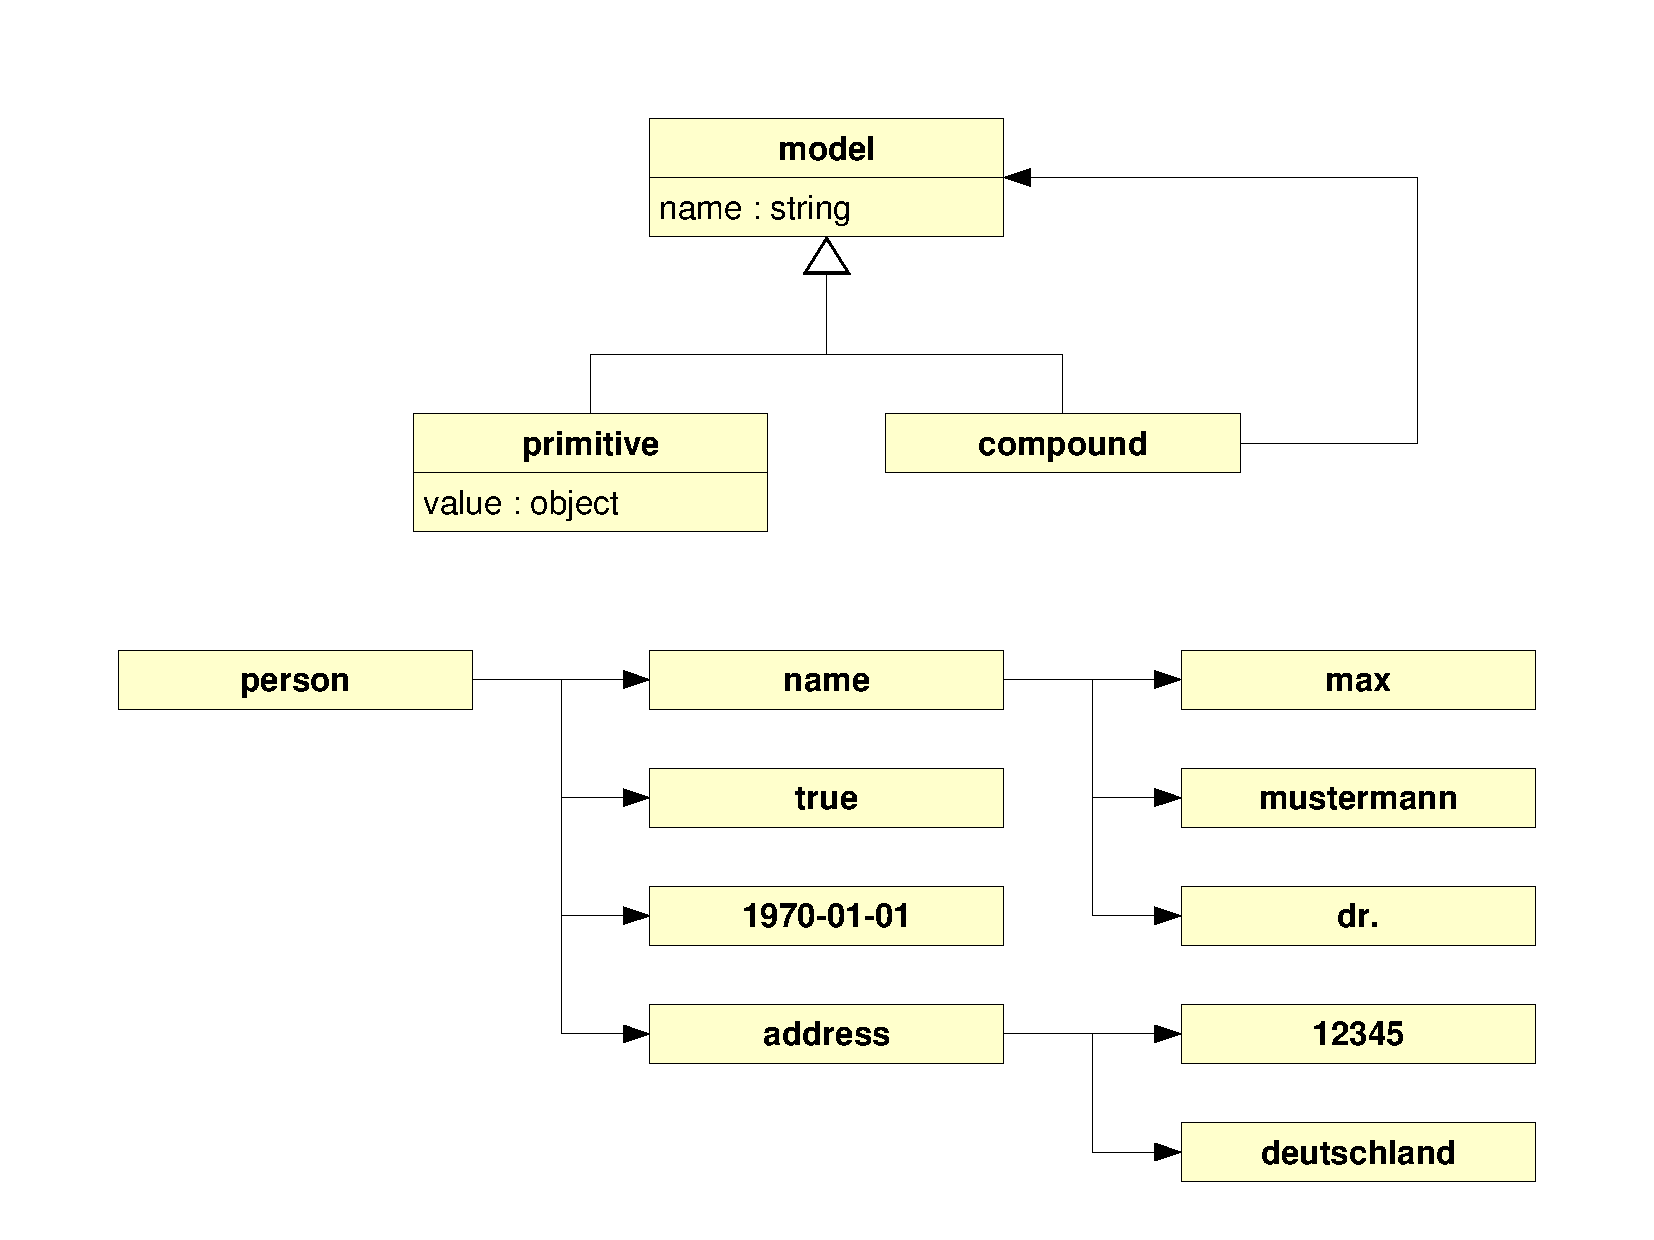
\includegraphics[scale=0.3,angle=-90]{graphic/hierarchical.pdf}
        \caption{Hierarchical Model Approach (adapted from \cite{archetypes})}
        \label{hierarchical_figure}
    \end{center}
\end{figure}

The upper half of figure \ref{hierarchical_figure} shows the \emph{Composite}
software pattern (section \ref{composite_heading}). Its classes do not contain
hard-coded attributes; two exceptions are the \emph{Primitive} class' attribute
\emph{value} and the \emph{Compound} class' dynamically extensible structure.
The structure may be a list, and it stores all of the compound's parts in it.
Parts may be primitiva or compounds themselves. As already proposed by the
\emph{Semi Structured Model} before, each part is identified by a name that is
unique within its compound. The diagram in the lower half of the figure clearly
shows the hierarchical tree structure of runtime instances.

The only open issue when using purely hierarchical models is that the semantics
-- the actual domain concepts -- is lost. Knowledge models, together with their
parts and meta information about these (position, size, colour, constraints --
as described in section \ref{human_thinking_heading}), thus need to be defined
somewhere else. The later section \ref{knowledge_representation_heading}
proposes a generic knowledge schema for doing this.

